\chapter{How fast is the galaxy rotating and what does it mean?}

\section{Introduction}
Throughout the past few weeks, you have been preforming labs which at times might have seemed disparate or only somewhat connected to each other. Now, you will bring all these concepts you have been working with in order to perform observations and make conclusions regarding the motion of the Milky Way. In this lab, you will be trying to measure how the rotational velocity of the milky way varies changes as you move away from the center. However, given the scale of the Milky Way, there is no way for us to directly observe its motion. However, we can use the motion of objects within the galaxy to calculate its rotational velocity. One useful object to do this are hydrogen clouds. In a previous lab you learned how shifts in frequency can be used to calculate the velocity of an object. In the case of hydrogen clouds, given that they emit at a very definite, known frequency we can calculate their velocity to a very high degree of accuracy. Moreover, given how common they are throughout the Milky Way, they can be used to make these measurements at many different points along the galactic plane. Using this data, you will calculate the rotational velocity of the galaxy at that point and create a rotation curve for the Milky Way. You will then use the curve to make inferences about the mass distribution of the Milky Way and see why dark matter is believed to play a role in its structure. 

\section{Learning Goals}
\begin{itemize}
	\item Use observation of hydrogen cloud velocities to determine motion of galactic plane
	
	\item Organize and present data in a logical and consistent manner and draw conclusions from it
	
	\item Interpret rotation curve data in order to make inferences about the mass distribution in the Milky Way
\end{itemize}

\section{Team roles}

\textbf{Decide on roles} for each group member. The available roles are:
\begin{itemize}
	\item Facilitator: ensures time and group focus are efficiently used
	\item Scribe: ensures work is recorded
	\item Technician: oversees apparatus assembly, usage
	\item Skeptic: ensures group is questioning itself
\end{itemize}

These roles can rotate each lab, and you will report at the end of the lab report on how it went for each role. If you have fewer than 4 people in your group, then some members will be holding more than one role. For example, you could have the skeptic double with another role. Consider taking on a role you are less comfortable with, to gain experience and more comfort in that role.

Additionally, if you are finding the lab roles more restrictive than helpful, you can decide to co-hold some or all roles, or think of them more like functions that every team needs to carry out, and then reflecting on how the team executed each function.

\section{Rotation of the Milky Way}

Our star system, the Solar System, resides within the Milky Way Galaxy. When we observe it directly, it looks like the following:
\begin{framed}
	\url{https://en.wikipedia.org/wiki/Milky_Way#/media/File:ESO-VLT-Laser-phot-33a-07.jpg}.
\end{framed}	
The galaxy has a spiral disc shape, and this image is looking towards the center of the galaxy. While we can't move outside our galaxy to take a picture of it, based on what we know, it probably looks like the artist's rendition here:
\begin{framed}
	\url{https://en.wikipedia.org/wiki/Galactic_coordinate_system#/media/File:Artist's_impression_of_the_Milky_Way_(updated_-_annotated).jpg}
\end{framed}
Locate the Sun in that image and notice the coordinate system that extends from it. This is the system of galactic longitude, shown as a schematic here:
\begin{framed}
	\url{https://en.wikipedia.org/wiki/Galactic_coordinate_system#/media/File:Galactic_coordinates.JPG}
\end{framed}
Throughout the galaxy, there are neutral hydrogen gas clouds in the spiral arms. The neutral hydrogen clouds emit light with a spectral line at a wavelength of 21 cm (frequency of 1420.4 MHz). Since they are all moving at different velocities, when we observe 21 cm line in the galactic disc (galactic latitude $b=0$), we see different distinct peaks at wavelengths close to 21 cm, caused by their differing Doppler shifts. So we can use Doppler shift to find the velocity of those clouds. A sample observation is found in Figure \ref{sgr:fig:hicloud1}.

\begin{figure}
	\centering
	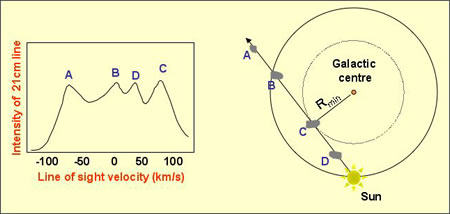
\includegraphics[width = 0.7\textwidth]{srt-galaxy-rotation/hicloud1}
	\caption{On the left, a graph of intensity vs line of sight velocity for 4 different gas clouds observed from Earth. The maximum line of sight velocity is from cloud C, since it's velocity orbiting the galactic center aligns with the line of sight. (Image from Swinburne University of Technology, \url{https://astronomy.swin.edu.au/cosmos/H/HI+cloud})}\label{sgr:fig:hicloud1}
\end{figure}

\subsection{Calculating Rotational Velocity}
When measuring the velocity of these objects, we have to keep in mind that we are moving relative to them. As such, we are not measuring their rotational velocity, but their velocity relative to us. We therefore have to do several calculations to get their orbital velocity. To do this calculation, we will need several components. First, we will need the velocity of the sun in the line of sight for the galactic longitude $l$. This is because the Sun is also moving along the galactic plane, and thus we need to be able to account for it in our measurements. We already know that the velocity of the Local Standard of Rest (the local stellar environment around the Sun) is 220km/s, so using some trigonometry, we can see that the line of sight velocity is given by
\begin{equation}
 V_\textrm{sun}(l) = (220\:\mathrm{km}/\mathrm{s}) \sin(l) \,.
\end{equation}
We also need to account for Earths rotation around the sun as well as relative motion of the solar system compared to the LSR. These are given to you by the SRT altogether as the VLSR or Velocity relative to the Local Standard of Rest. From the graph generated by the telescope, we simply need the maximum VLSR, as it corresponds to the hydrogen cloud directly in our line of sight. The circular velocity of the cloud can thus be obtained by
\begin{equation}
 V_c(r) = v_\textrm{max} (l) + v_\textrm{sun}(l) \,.
\end{equation}
Finally, for the final data processing, you will need the distance of that cloud from the center of the galaxy. Once again, from the geometry of the graph above, we can see that this can be found from the distance of the Sun to the center $r_0 = 8.5\textrm{kpc}$ (kiloparsec) and the galactic longitude $l$. The distance is then given by
\begin{equation}
 r = r_0 \sin(l)
\end{equation}

% Change gamma to l, parenthesis around 220km, spacing between number and unit use example on slack



\subsection{Goal}
Measure the rotational velocity of the galactic plane along different orbital radii, create a rotation curve for the milky way and infer the mass distribution from it.
\subsection{Equipment}
\begin{itemize}
	\item LAB sky survey: \url{https://www.astro.uni-bonn.de/hisurvey/AllSky_profiles/}
	\item Small Radio Telescope
\end{itemize}


\subsection{Calibration}
Before you begin your observations of the hydrogen clouds, you have to calibrate the telescope similarly to how you did in the previous lab. However, this time you have two options for calibrating: The offset frequency method and the off-source method. The two methods are described below.

\subsubsection{Offset Frequency Method (recommended)}
\begin{enumerate}
	\item Move the telescope to one of the locations you want to measure on the galactic plane (marked by the Gxxx)
	
	\item Change the telescope frequency to 1423MHz in mode 4 and clear the screen. This frequency is far enough from the hydrogen line that you will only be measuring the receiver noise and thermal background.
	
	\item Once you have cleared the output, select "Cal" to begin the calibration procedure. Note the $T_\textrm{sys}$ and $T_\textrm{rec}$
	
	\item Clear the output again and repeat the calibration procedure 2-3 times or until you note a stable $T_\textrm{sys}$ and $T_\textrm{rec}$. 
\end{enumerate}

\subsubsection{Off-Source Method}

\begin{enumerate}
	\item Point the telescope to some location far away from the galactic plane (away from the labeled sources). 
	
	\item Change the receiver frequency to 1420.4MHz in mode 4 and clear the output
	
	\item Once you have cleared the output, select "Cal" to begin the calibration procedure. Note the $T_\textrm{sys}$ and $T_\textrm{rec}$.
	
	\item  Clear the output again and repeat the calibration procedure 2-3 times or until you not a stable $T_\textrm{sys}$ and $T_\textrm{rec}$. \textbf{If there is a major hydrogen source in your pointing, the calibration will not work. Look out for strong spectral features when calibrating to make sure you are not pointed at a hydrogen source. If this were the case, try moving the telescope. You likely wont find a spot without any hydrogen emissions, but you can try to avoid significant sources. If not try the offset frequency method instead.} 
\end{enumerate}


\subsection{Steps}

\begin{steps}
	\item In the control panel, the positions of different Galactic longitudes along
	the equator are indicated by Gxxx (where xxx is in degrees). If you see
	longitude of 90 degrees and smaller, start at the longitude of 90
	degrees and work your way down to the smallest longitude you can
	observe down to zero of the center of our Galaxy (coincident with the
	source named Sgr A). If you cannot observe longitudes smaller than
	90 degrees observe one or two longitudes that are up in the sky. Note
	that galactic coordinates labeled in the SRT display can be pointed to
	by clicking on them – for the rest you have to estimate (or look up) the
	Az El of the desired longitude on the galactic plane. %add framing comment 
	
	\item Move to your first pointing and press Clear button to clear the spectrum accumulated by the SRT.
	
	\item  Set the frequency to 1420.4MHz with mode  4 by typing in ``1420.4 4'' and obtain the spectrum for the galactic longitudes visible in the sky by integrating for 10--20 seconds (or longer) along the same pointing.
	
	\item After integration click on the spectrum window to get a detailed plot of
	the spectrum in a separate window. You will see emission flux in units of kelvins (K) as a
	function of frequency and VSLR. Based on your understanding of how frequencies are affected by Doppler shift, estimate that maximum velocity of the clouds visible in the spectrum. 
	
	\item Record the spectrum by taking a screenshot of the spectrum plot. If necessary, crop the image in your preferred image editor such that only the spectrum viewer is visible. Your screenshot should look something like Figure \ref{sgr:fig:spec-example}.
\end{steps}%
\begin{figure}
	\centering
	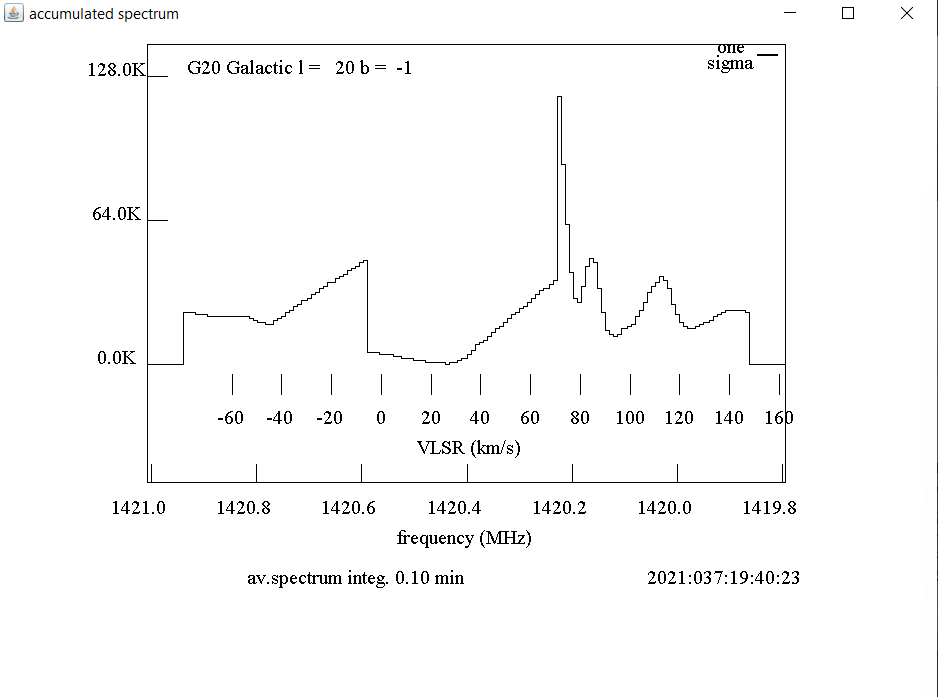
\includegraphics[width = 0.7\textwidth]{srt-galaxy-rotation/spectrum_ex}
	\caption{An example of a good capture of the spectrum plot. Note the different clear peaks that are seen.} 
	\label{sgr:fig:spec-example}
\end{figure}%
\begin{steps}
	\item Proceed to the next Galactic longitude available for observation. Press Clear button to clear the spectrum before you make observation at
	each new longitude. Record longitude and spectrum. Given the limited time, each group should do 2-3 observations and supplement the rest of the data either by sharing with the other groups or using the LAB survey described below.%rewrite given current situaton
	
	\item After you have preformed all the possible observations, open the link to the LAB sky survey provided in the equipment section. 
	
	\item In the search box, make sure that only the LAB survey box is checked and that Dec is always at 0. Figure \ref{sgr:fig:lab-box} demonstrates how the display should look like.
\end{steps}

\begin{figure}
	\centering
	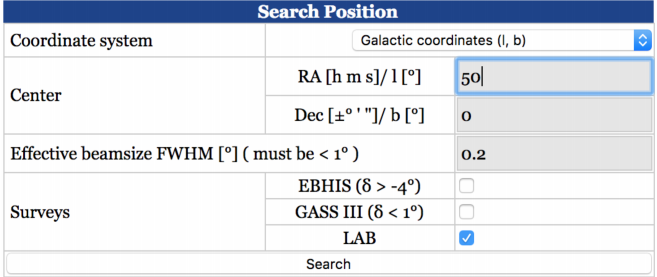
\includegraphics[width = 0.7\textwidth]{srt-galaxy-rotation/LAB_box}
	\caption{The input form for accessing the LAB spectra. Dec is always set to 0, only LAB is selected, FWHM is set to 0.2 and galactic coordinate system is used.} 
	\label{sgr:fig:lab-box}
\end{figure}

\begin{steps}
	\item Obtain spectra from the LAB survey along the galactic equator for the
	longitudes that you could not observe with SRT. Measure the
	maximum radial velocity, Vmax (note these will be max positive for
	longitudes 10 to 90 deg. and max negative for longitudes -10 to -90
	deg.). You will note that the spectrum does not provide a clean
	maximum velocity. Try to think about the best way to measure
	maximum velocity, given that you may be observing several hydrogen clouds all in a line, moving at different velocities.
	
%	\item Re-observe one of the longitudes that you have observed with the SRT
%	and compare the spectrum you get from the LAB survey to that you
%	have obtained with the SRT. Discuss any similarities and differences
%	that you may find. 
	
	\item Assuming a distance from the Sun to the galactic center of 8.5 kpc and
	a circular velocity of 220 km/s at this radius, make a spreadsheet that follows the template in Table \ref{sgr:tab:data} with the
	results of your calculations using your measurements of $v_\textrm{max}$ and
	equations above.
	
	\item Plot the orbital velocity versus the distance from the center in kpc using your plotting program of choice. \textbf{Include this graph in your report.}
	
	\item From the rotation curve you obtain, how do you expect the matter to be distributed in the galaxy? \textbf{Record your answer.}
	
	\item In our own solar system, the sun makes up most of the mass. As such, a safe assumption to make is that the mass in a given region of our galaxy is roughly proportional to its brightness (the brighter a region, the more stars and therefore the more mass there is). The brightness of our galaxy as a function of the radius can be roughly modeled using the equation $I(r) = e^{-r/2.1}$. In Desmos online graphing calculator, plot the equation. 
	
	\item Take a screenshot of the graph you obtain. Describe the behavior of the graph. How does brightness change as you move farther away from the center of the milky way?
	
	\item Using the assumption above that mass is roughly proportional to brightness, how would you expect mass to be distributed in the Milky way? How does it compare to what you found from the rotation curve. 
	
	\item Think of possible explanations for the discrepancy between the distribution of mass suggested by the brightness curve and the distribution suggested by the rotation curve. Think about the assumptions that went into the equations and how you came to your original conclusions for each curve. \textbf{Record your discussion.}
	
	
\end{steps}

\begin{table}
	\centering
	\begin{tabular}{|p{3cm}|p{3cm}|p{3cm}|p{3cm}|p{3cm}|}
		\toprule
		Galactic Longitude (degrees) & Tangential Distance r (kpc) & Maximum VLSR $v_\textrm{max}$ (km/sec) & Line of Sight Solar Velocity $V_\textrm{sun}$ (km/sec) & Circular Velocity $v_c$ (km/sec) \\ \midrule 10 & & & & \\ \midrule 20 &&&& \\ \midrule 30 &&&&\\ \midrule 40 &&&& \\ \midrule 50 &&&& \\ \midrule 60 &&&& \\ \midrule 70 &&&& \\ \midrule 80 &&&& \\ \midrule 90 &&&& \\ \midrule -10 &&&& \\ \midrule -20 &&&& \\ \midrule -30 &&&& \\ \midrule -40 &&&& \\ \midrule -50&&&& \\ \midrule -60 &&&& \\ \midrule -70 &&&& \\ \midrule -80 &&&& \\ \midrule -90 &&&& \\ \bottomrule
	\end{tabular}
	\caption{Data Table for measurement of the rotation velocity of the Galaxy}\label{sgr:tab:data}
\end{table}

\section{Report Checklist}

Include the following in your lab report. See Appendix~\ref{cha:lab-report-format} for formatting details. Each item below is worth 10 points.

\begin{enumerate}
	\item Calibration details - method used, sequence of Tsys and Trec observed.
	\item Emission flux vs frequency graphs for your group's observations and description of maximum velocity determination
	\item Completed data table with SRT observations marked, and your group observations marked
	\item Flux vs frequency graph for one of the longitudes from the LAB survey
	\item Data from LAB survey included in data table
	\item Graph of your measured Milky Way rotation curve
	\item Inference of matter distribution from light curve
	\item Inference of matter distribution from rotation curve
	\item Re-evaluation of assumptions and possible explanation for discrepancies between matter distributions.
	\item A 100--200 word reflection on group dynamics and feedback on the lab manual. Address the following topics: who did what in the lab, how did you work together, how group roles functioned, what successes and challenges in group functioning did you have, and what would you keep and change about the lab write-up?
\end{enumerate}












